\section{Máquinas de vector soporte '\textit{Support Vector Machines}'}
\label{resultados:svm}

\subsection{Características de los conjuntos de datos a analizar}
\label{resultados:rf_caracteristicas}
Al realizar las mismas transformaciones que para el caso de \hyperref[resultados:knn_caracteristicas]{K-NN}, las características de los conjuntos de datos son las mismas.

\subsection{(Caso de estudio 1) Resultados del entrenamiento con el Conjunto de datos solo con atributo utilidad definido y escogiendo los atributos que nos ha indicado como relevantes el \hyperref[result:pca_case2]{caso de estudio 2} del PCA}

\paragraph{}
Para realizar el entrenamiento y posterior validación del modelo de {Máquinas de vector soporte '\textit{Support Vector Machines}' es necesario decidir que funciones \textit{kernel} vamos a utilizar para entrenar el modelo. Según la función \textit{kernel} que escojamos, influirá en el comportamiento y resultados del modelo. Para realizar el entrenamiento nos ayudaremos de la librería \textit{svm} del paquete \textit{sklearn} que dispone del modelo de clasificación\cite{ref:svm_sklearn_svc} ya implementado con las funciones \textit{kernel} '\textit{lineal}', '\textit{polynomial}', '\textit{radial (rbf)}' y '\textit{sigmoid}'\cite{ref:svm_kernels_sklearn} disponibles. Este paquete también permite poder implementar nuestras propias funciones \textit{kernel} pero descartamos esta opción por el tiempo que implicaría realizar ese desarrollo, que provocaría que nos saliéramos del tiempo limite para la presentación de este análisis.

\paragraph{}
Antes de realizar el entrenamiento comparativo, dibujaremos en un gráfico todos los valores siendo 'Y' un atributo en concreto del dataset y 'X' el atributo a predecir. Dibujaremos todos los atributos en el mismo gráfico con la idea de intentar dibujar un hiperplano lineal (división de valores) que nos ayude a poder clasificar los valores del campo utilidad en base los atributos del dataset. Como podemos ver en la figura \ref{svmDistribution} esta división no es posible a simple vista ya que los resultados del campo '\textit{utilidad}' están distribuidos sobre todo el plano de 'X' por lo que descartaremos la utilización de la función kernel \textit{lineal} y probaremos con el resto de funciones.

\begin{figure}[!htb]
  \centering
    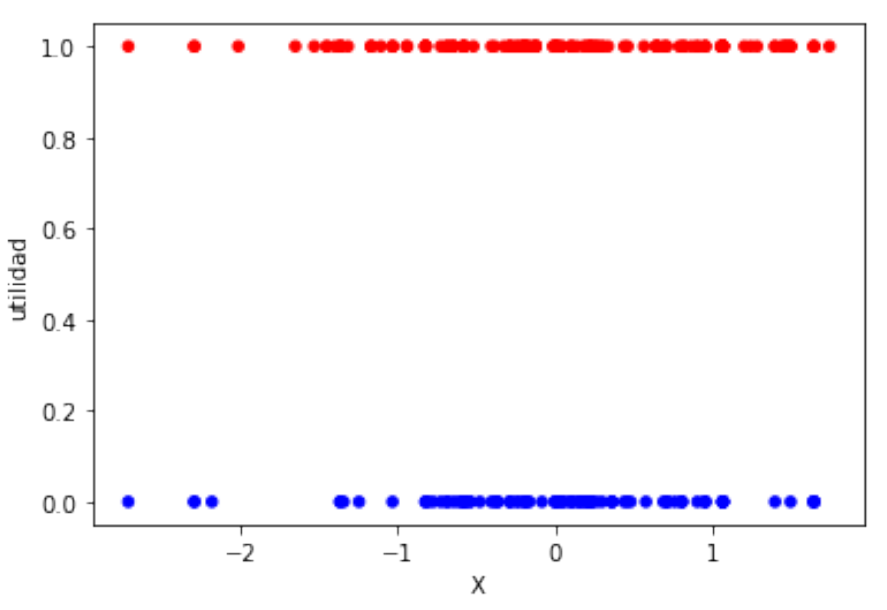
\includegraphics[width=0.4\textwidth]{images/resultados_svm_distribucion.png}
    \caption{Distribución de los valores del dataset respecto al atributo \textit{utilidad} para el caso de estudio 1.}
  \label{svmDistribution}
\end{figure}

\paragraph{}
Para explorar los hiper parámetros que necesitaremos, nos ayudaremos de la función '\textit{RandomizedSearchCV}' de la librería '\textit{sklearn.model\_selection}' que nos ayudara a ejecutar varias veces el modelo con distintos valores. Para el \textbf{parámetro C}, que indica el valor de penalización de los errores en la clasificación (indica el compromiso entre obtener el hiperplano con el margen más grande posible y clasificar el máximo número de ejemplos correctamente). Probaremos \textbf{valores aleatorios distribuidos uniformemente entre 1 y 500}. Para el parámetro \textbf{gamma} nos basaremos en la propia documentación del modelo que nos indica que utilizando un rango de \textbf{valores aleatorios distribuidos uniformemente entre $10^{-3}$ y $10^{3}$} suele ser suficiente para encontrar un resultado optimo. Puede consultar el código para la realización de estos entrenamientos en el anexo (\nameref{anx06:svm1}).

\paragraph{}
Una vez realizado el entrenamiento podemos ver (como se aprecia en la figura \ref{svmTrainCase1}) que el modelo con más precisión es el '\textit{radial (rbf)}'. Pero si analizamos su comportamiento con el conjunto de datos de test vemos que su precisión baja obteniendo un \textbf{porcentaje de acierto de cerca del 54\%}.

\paragraph{}
Si mostramos la matriz de confusión\cite{ref:confusion_matrix} (figura \ref{svmCMCase1}) para poder ver que porcentaje de aciertos tiene el modelo con el conjunto de test, vemos que tiene un \textbf{porcentaje de aciertos muy bajo} siendo el resultado totalmente aleatorio.

\begin{figure}[!htb]
  \centering
		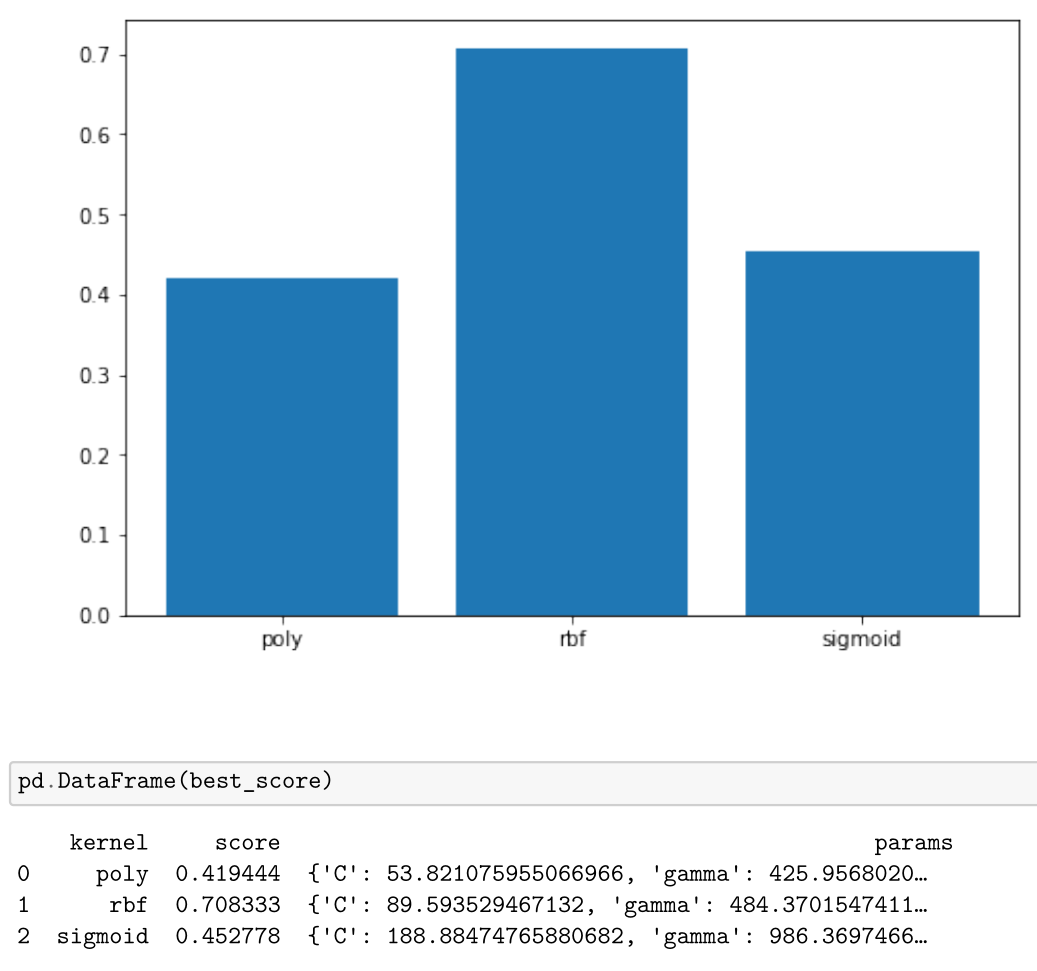
\includegraphics[width=0.6\textwidth]{images/resultados_svm_ent_conjunto1.png}
		\caption{Resultado del entrenamiento de las diferentes funciones \textit{kernel} para el caso de estudio 1.}
  \label{svmTrainCase1}
\end{figure}

\begin{figure}[!htb]
  \centering
	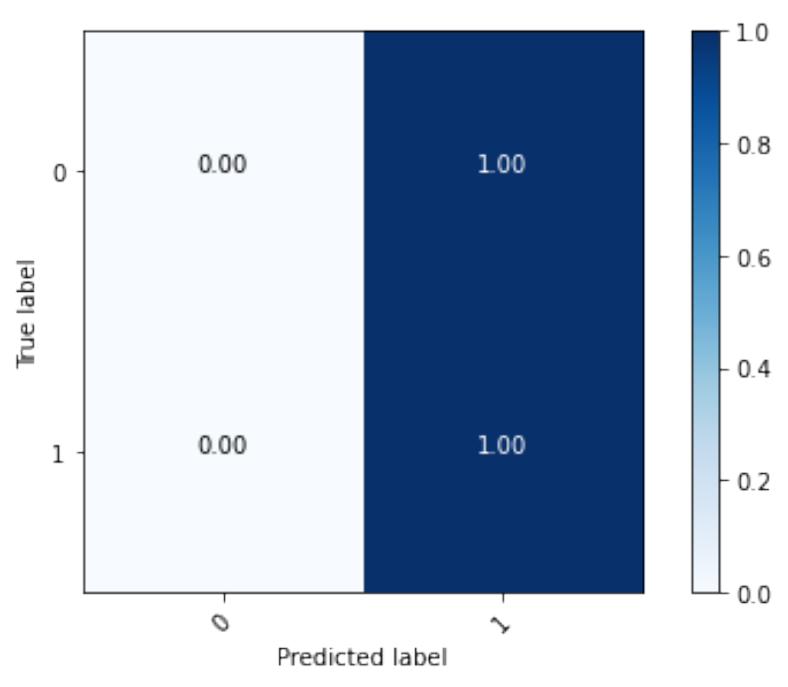
\includegraphics[width=0.4\textwidth]{images/resultados_svm_cm_conjunto1.png}
	\caption{Matriz de confusión para el modelo \textit{SVM} con la función \textit{kernel} radial para el caso de estudio 1.}
  \label{svmCMCase1}
\end{figure}

\subsection{(Caso de estudio 2) Conjunto de datos solo con atributo utilidad definido, añadiendo el mes y año del artículo, eliminando los atributos \textit{gender} y artículo y expandiendo el atributo \textit{respuesta.pubmed\_keys}. También escogemos solo los atributos que nos ha indicado como relevantes el \hyperref[result:pca_case3]{caso de estudio 3} del PCA}

\paragraph{}
Igual que en el caso anterior, antes de realizar el entrenamiento del modelo, dibujaremos en un gráfico todos los valores siendo 'Y' un atributo en concreto del dataset y 'X' el atributo a predecir. Igual que en el caso anterior (como podemos ver en la figura \ref{svmDistributionCase2}) no es posible hacer la división del hiperplano lineal (división de valores) que nos ayude a poder clasificar los valores del campo utilidad a simple vista, ya que los resultados del campo '\textit{utilidad}' están distribuidos sobre todo el plano de 'X' por lo que descartaremos la utilización de la función \textit{kernel} \textit{lineal} y probaremos con el resto de funciones.

\begin{figure}[!htb]
  \centering
    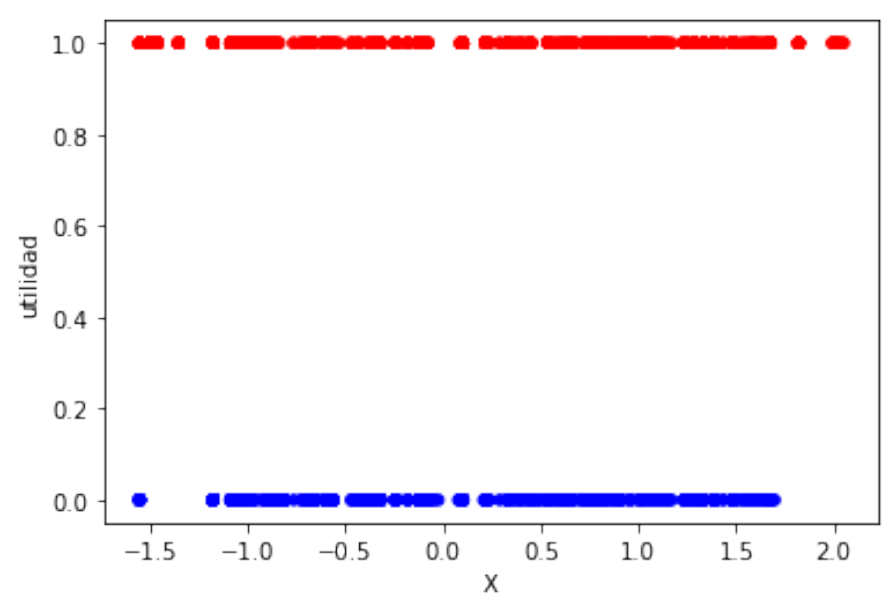
\includegraphics[width=0.4\textwidth]{images/resultados_svm_distribucion_conjunto2.png}
    \caption{Distribución de los valores del dataset respecto al atributo \textit{utilidad} para el caso de estudio 2.}
  \label{svmDistributionCase2}
\end{figure}

\paragraph{}
Para explorar los hiper parámetros que utilizaremos los mismos rangos que los utilizados para el caso de estudio 1, para así poder comparar los resultados. \textbf{Nota:} Para la función \textit{kernel polinomial} descartamos el poder realizar el entrenamiento por problemas de rendimiento, debido a que el modelo tardaba excesivo tiempo en realizar su entrenamiento (más de 3 días). Puede consultar el código para la realización de estos entrenamientos en el anexo (\nameref{anx06:svm2}).

\paragraph{}
Una vez realizado el entrenamiento podemos ver (como se aprecia en la figura \ref{svmTrainCase2}) que el modelo con más precisión es el '\textit{radial (rbf)}'. Ademas si analizamos su comportamiento con el conjunto de datos de test vemos que su precisión mantiene el \textbf{porcentaje de acierto de cerca del 89\%}.

\paragraph{}
Si mostramos la matriz de confusión\cite{ref:confusion_matrix} (figura \ref{svmCMCase2}) para poder ver que porcentaje de aciertos tiene el modelo con el conjunto de test, vemos que tiene un \textbf{porcentaje de aciertos bastante aceptable}.

\begin{figure}[!htb]
  \centering
	    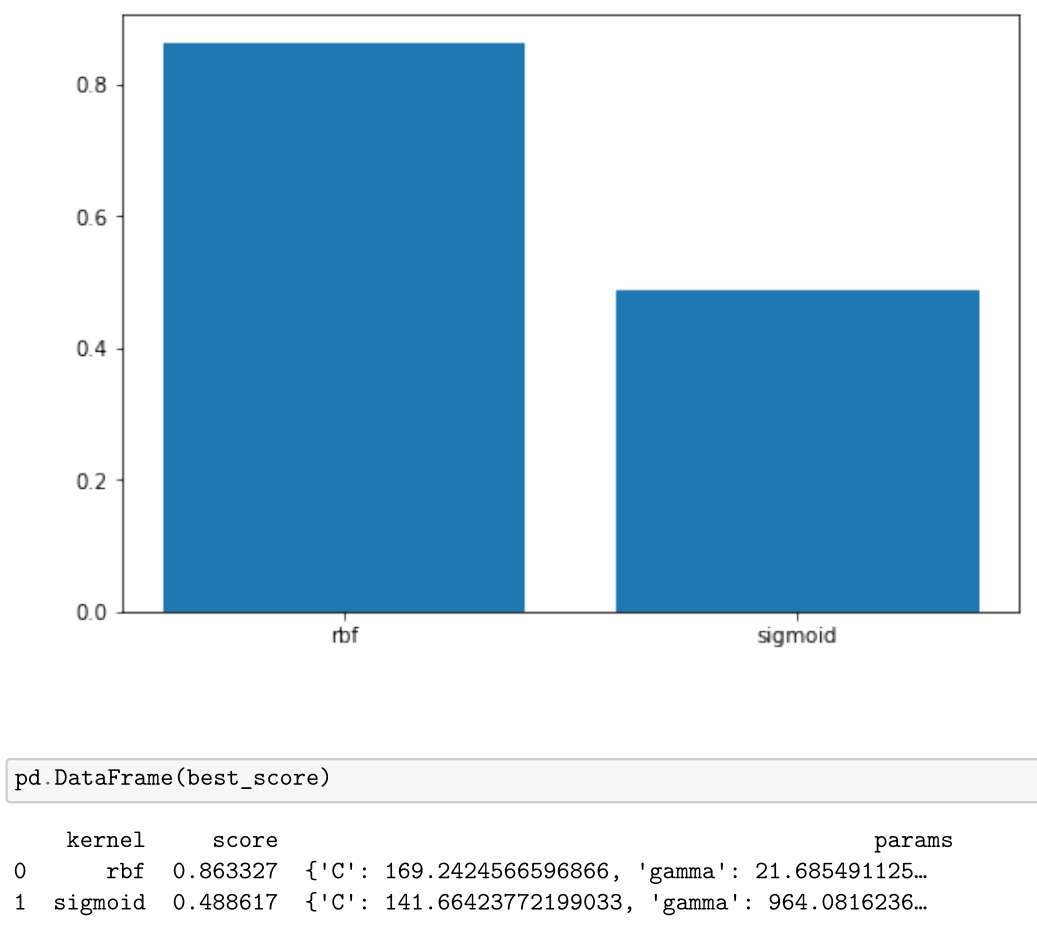
\includegraphics[width=0.6\textwidth]{images/resultados_svm_ent_conjunto2.png}
    	\caption{Resultado del entrenamiento de las diferentes funciones \textit{kernel} para el caso de estudio 2.}
	\label{svmTrainCase2}
\end{figure}

\begin{figure}[!htb]
  \centering
		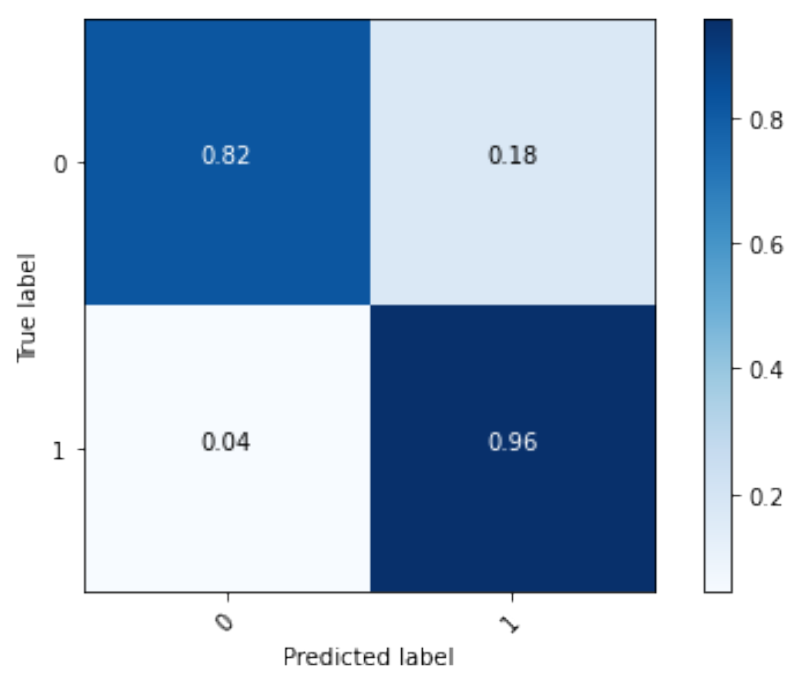
\includegraphics[width=0.4\textwidth]{images/resultados_svm_cm_conjunto2.png}
		\caption{Matriz de confusión para el modelo \textit{SVM} con la función \textit{kernel} radial para el caso de estudio 2.}
		\label{svmCMCase2}  
\end{figure}

\paragraph{}
En este caso, podemos apreciar que el \textbf{caso 2 se ajusta a unos resultados aceptables} ya que esta lo suficientemente ajustado para que de resultados razonables sin estar sobreajustado\cite{ref:knn_overfiting}. Por lo que recomendamos al cliente como posible modelo final el modelo de Máquinas de vector soporte '\textit{Support Vector Machines}' con la función \textit{kernel} '\textit{radial (rbf)}' aplicando las transformaciones al conjunto de datos realizado en el caso de estudio 2.
